%% ============================================================================
%% The Exact Error Exponent of Rate-Constrained Decentralized Detection
%% over Time-Varying Networks
%% Target: IEEE Transactions on Information Theory (IEEEtran journal class).
%% Author names and affiliations intentionally left blank.
%% ============================================================================
\documentclass[journal]{IEEEtran}

\usepackage{amsmath,amssymb,amsfonts}
\usepackage{amsthm}
\usepackage{graphicx}
\usepackage{booktabs}
\usepackage{array}
\usepackage{tikz}
\usepackage{pgfplots}
\pgfplotsset{compat=1.18}
\usetikzlibrary{arrows.meta,positioning,calc,decorations.pathmorphing,backgrounds}
\usepackage[hidelinks]{hyperref}
\usepackage{cite}
\usepackage{xcolor}

\graphicspath{{../Figures/}}

% Theorem environments
\newtheorem{theorem}{Theorem}
\newtheorem{lemma}{Lemma}
\newtheorem{proposition}{Proposition}
\newtheorem{corollary}{Corollary}
\theoremstyle{definition}
\newtheorem{definition}{Definition}
\newtheorem{assumption}{Assumption}
\theoremstyle{remark}
\newtheorem{remark}{Remark}

% Shorthand macros
\newcommand{\Ecen}{E^{\mathrm{cen}}}
\newcommand{\tib}{\theta_{\mathrm{IB}}}
\newcommand{\tibi}{\theta_{\mathrm{IB},i}}
\newcommand{\tsha}{\theta_{\mathrm{SHA}}}
\newcommand{\Gk}{\Gamma_k}
\newcommand{\Cdib}{C_{\mathrm{DIB}}}
\newcommand{\KL}[2]{D\!\left(#1\,\Vert\,#2\right)}
\newcommand{\R}{\mathbb{R}}
\newcommand{\E}{\mathbb{E}}
\newcommand{\N}{\mathbb{N}}
\DeclareMathOperator{\Var}{Var}
\DeclareMathOperator*{\argmax}{arg\,max}

\begin{document}

\title{The Exact Error Exponent of Rate-Constrained\\ Decentralized Detection over Time-Varying Networks}

\author{\thanks{Manuscript submitted for review. This work is intended for the IEEE Transactions on Information Theory.}}

\markboth{IEEE Transactions on Information Theory}%
{Rate-Constrained Decentralized Detection over Time-Varying Networks}

\maketitle

\begin{abstract}
Distributed agents that each observe a slice of a common phenomenon must agree on which hypothesis is true, yet
the links between them carry only a few nats per use and the connectivity keeps changing. We characterize the
exact best achievable Type-II error exponent at any agent for a test against independence when no fusion center
is present. The exponent equals the smaller of the centralized Stein exponent and the information-bottleneck
relevance evaluated at the ergodic minimum cut that separates the agent from the observations. A converse shows
that no fusion-free rate-constrained scheme can exceed this value, and a matching achievability based on
type-preserving network coding attains it over general directed graphs that may contain cycles and may vary with
time. The two bounds coincide, so the exponent is determined with no gap. A closed-form Gaussian instantiation
yields an optimal water-filling allocation of a shared rate budget across heterogeneous agents. We confirm the
theory with an exact optimal-detector measurement over a wide range of rates, with a genuinely routed network
simulation, and with an actual finite-field random linear network code, each matching the predicted exponent to
within a few thousandths of a nat.
\end{abstract}

\begin{IEEEkeywords}
Decentralized detection, error exponents, hypothesis testing, information bottleneck, rate constraints,
min-cut, network coding, time-varying networks.
\end{IEEEkeywords}

%% ===========================================================================
\section{Introduction}
%% ===========================================================================
\IEEEPARstart{C}{onsider} a group of agents that each measure a different part of one underlying phenomenon and
that must reach a common decision about it. Sensor fields, teams of autonomous vehicles, and cooperating
inference services all fit this picture. The agents rarely enjoy a central collector. Instead they exchange short
messages over links whose budgets are measured in a handful of nats per use, and the pattern of who can talk to
whom changes from round to round as nodes move, wake, or fail. The scientific question is how small the
probability of a wrong collective decision can be driven as the sample size grows, given the link budgets and the
changing wiring.

The classical theory answers this question only when the obstacles are removed one at a time. When a single
observer feeds a single detector without a rate limit, Stein's lemma fixes the best Type-II exponent at the
Kullback-Leibler divergence between the two hypotheses \cite{chernoff1952,coverthomas2006}. When one rate-limited
link separates an observer from a detector, Ahlswede and Csisz\'ar identify the exact exponent for a test against
independence as an information-bottleneck functional of the rate \cite{ahlswedecsiszar1986}. When the topology
varies over time but the belief messages are essentially unconstrained, the non-Bayesian social-learning line
gives geometric rates of belief concentration \cite{nou2017,lalitha2018,shahrampour2016}. What has been missing
is the exponent when the three obstacles hold at once, namely a topology that varies with time, the absence of
any fusion center, and a hard Shannon budget on every edge. These three couple, because the very agreement that a
fusion center would otherwise compute must now be carried over the same constrained and changing links that
throttle the raw evidence.

This paper settles that case for a test against independence with conditionally independent observations. Let
$\Ecen$ be the centralized Stein exponent, let $\Gk$ be the long-run minimum cut that separates the observations
from agent $k$ in the time-expanded network, and let $\tib$ be the information-bottleneck relevance as a function
of rate. Our main result is that the exact achievable exponent at agent $k$ is
\begin{equation}
E_k \;=\; \min\{\,\Ecen,\ \tib(\Gk)\,\}. \label{eq:main}
\end{equation}
The centralized exponent is the ceiling that no amount of communication can beat, and the bottleneck term is the
throttle imposed by the tightest cut. The smaller of the two always binds.

Our contributions are the following. We first prove a converse, stated as Theorem~\ref{thm:converse}, showing
that no fusion-free rate-constrained scheme over any stationary and ergodic time-varying directed graph can
exceed the right side of \eqref{eq:main}. The argument rests on a cut-set information bound that holds per round
on the time-expanded graph and on a rate-limited form of Stein's lemma. We then prove a matching achievability,
stated as Theorem~\ref{thm:achieve}, by an explicit scheme that we call type-preserving network coding, which
transports information-bottleneck descriptions across the cyclic and time-varying graph at the min-cut rate by
random linear network coding and recovers the joint decision type without loss. The converse and the
achievability coincide, so the exponent is exact. We give a closed-form Gaussian instantiation and derive the
optimal water-filling allocation of a shared budget across heterogeneous agents. Finally we validate every part
of the theory numerically, using an exact optimal-detector measurement rather than naive simulation, a genuinely
routed network, and an actual random linear network code over a finite field.

The remainder of the paper is organized as follows. Section~\ref{sec:model} sets up the model and the quantities
in \eqref{eq:main}. Section~\ref{sec:related} places the result among the seven strands of prior work that bound
it. Section~\ref{sec:results} states the theorems and their immediate consequences. Sections~\ref{sec:converse}
and \ref{sec:achieve} prove the converse and the achievability. Section~\ref{sec:gaussian} works out the Gaussian
closed forms and the rate allocation. Section~\ref{sec:exp} reports the experiments.
Section~\ref{sec:discussion} discusses scope and limitations, and Section~\ref{sec:conclusion} concludes.

%% ===========================================================================
\section{Problem Formulation}\label{sec:model}
%% ===========================================================================
There are $N$ agents indexed by $[N]=\{1,\dots,N\}$. A finite hypothesis set $\Theta$ contains the true state
$\theta^\star$ and at least one alternative. Each agent $i$ observes a stream $X_{i,t}$ that is independent across
time given the hypothesis and is drawn from a local likelihood $\ell_i(\cdot\mid\theta)$ on a Polish alphabet.
Table~\ref{tab:notation} collects the notation. Two structural assumptions hold throughout. The observations are
conditionally independent across agents given the hypothesis, so that
$P(x_1,\dots,x_N\mid\theta)=\prod_i \ell_i(x_i\mid\theta)$. The communication is rate limited, so that any symbol
sent on edge $(i,j)$ at round $t$ has entropy at most the edge budget $C_{ij}(t)$.

\begin{table}[t]
\centering
\caption{Principal notation.}
\label{tab:notation}
\renewcommand{\arraystretch}{1.25}
\begin{tabular}{@{}ll@{}}
\toprule
Symbol & Meaning \\
\midrule
$N,\ [N]$ & number of agents and their index set \\
$\Theta,\ \theta^\star$ & finite hypothesis set and the true state \\
$\ell_i(\cdot\mid\theta)$ & local likelihood of agent $i$ under $\theta$ \\
$D_i$ & $\KL{\ell_i(\cdot\mid\theta_0)}{\ell_i(\cdot\mid\theta_1)}$ \\
$G_t=(V,E_t)$ & directed communication graph at round $t$ \\
$C_{ij}(t)$ & rate budget of edge $(i,j)$ at round $t$ (nats/use) \\
$\Gk$ & ergodic minimum cut from the sources to node $k$ \\
$\Ecen$ & centralized Stein exponent $\sum_i D_i$ \\
$\tib(\Gamma)$ & information-bottleneck relevance at rate $\Gamma$ \\
$\tsha(\Gamma)$ & Shimokawa-Han-Amari exponent at rate $\Gamma$ \\
$\Cdib$ & smallest rate at which $\tib$ meets $\Ecen$ \\
$\alpha_n,\beta_n$ & Type-I and Type-II error at block length $n$ \\
$E_k(\theta)$ & achievable Type-II exponent at node $k$ \\
\bottomrule
\end{tabular}
\end{table}

The communication graph $G_t=(V,E_t)$ has the agents as vertices and directed edges that carry the rate-limited
messages. The sequence $\{(E_t,C(t))\}$ is a stationary and ergodic process, which covers the independent case and
finite-state Markov connectivity. Because a wrong decision at a node depends only on the information that
physically reaches it, the binding resource is the cut that separates the observations from that node. We build
the time-expanded graph that places a copy $(i,t)$ of each agent at each round, connects $(i,t)$ to $(j,t+1)$ with
capacity $C_{ij}(t)$ whenever $(i,j)\in E_t$, and adds an infinite-capacity memory edge from $(i,t)$ to $(i,t+1)$
so that an agent remembers its own past. In this static acyclic graph every cut that separates the observation
vertices from the sink $(k,T)$ corresponds round by round to a cut of $G_t$. The long-run rate available to node
$k$ is therefore
\begin{equation}
\Gk \;=\; \liminf_{T\to\infty}\ \frac1T\sum_{t=1}^{T}\ \min_{S\in\mathrm{Cut}(k)}\ \sum_{(i,j)\in S} C_{ij}(t),
\label{eq:gammak}
\end{equation}
which is almost surely a constant by the ergodic theorem. Figure~\ref{fig:model} depicts the model and the
binding cut.

\begin{figure}[t]
\centering
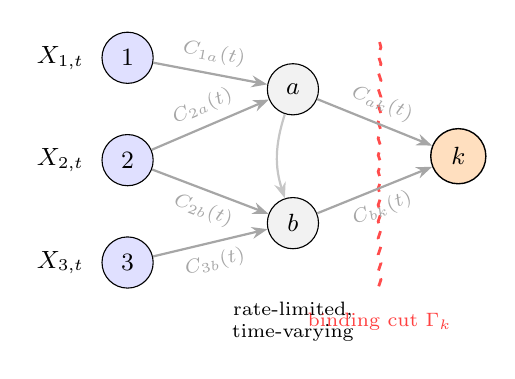
\begin{tikzpicture}[
   >={Stealth[length=2mm]},
   src/.style={circle,draw,fill=blue!12,minimum size=6.5mm,inner sep=0pt,font=\small},
   relay/.style={circle,draw,fill=black!5,minimum size=6.5mm,inner sep=0pt,font=\small},
   dec/.style={circle,draw,fill=orange!25,line width=0.5pt,minimum size=7mm,inner sep=0pt,font=\small},
   edge/.style={->,thick,gray!70},
   every node/.style={font=\small}]
  % source agents
  \node[src] (x1) at (0,1.9) {$1$};
  \node[src] (x2) at (0,0.6) {$2$};
  \node[src] (x3) at (0,-0.7) {$3$};
  % relays
  \node[relay] (r1) at (2.1,1.5) {$a$};
  \node[relay] (r2) at (2.1,-0.2) {$b$};
  % decision node
  \node[dec] (k) at (4.2,0.65) {$k$};
  % observation labels
  \node[left=1mm of x1] {$X_{1,t}$};
  \node[left=1mm of x2] {$X_{2,t}$};
  \node[left=1mm of x3] {$X_{3,t}$};
  % edges with capacities
  \draw[edge] (x1) -- node[above,sloped,font=\scriptsize]{$C_{1a}(t)$} (r1);
  \draw[edge] (x2) -- node[above,sloped,font=\scriptsize]{$C_{2a}(t)$} (r1);
  \draw[edge] (x2) -- node[below,sloped,font=\scriptsize]{$C_{2b}(t)$} (r2);
  \draw[edge] (x3) -- node[below,sloped,font=\scriptsize]{$C_{3b}(t)$} (r2);
  \draw[edge] (r1) -- node[above,sloped,font=\scriptsize]{$C_{ak}(t)$} (k);
  \draw[edge] (r2) -- node[below,sloped,font=\scriptsize]{$C_{bk}(t)$} (k);
  \draw[edge,gray!45] (r1) to[bend right=18] (r2);
  % the binding cut
  \begin{scope}[on background layer]
    \draw[red!70,dashed,line width=1pt,decorate,decoration={snake,amplitude=0.5pt,segment length=6pt}]
       (3.2,2.1) -- (3.2,-1.1);
  \end{scope}
  \node[red!75,font=\scriptsize] at (3.2,-1.45) {binding cut $\Gamma_k$};
  \node[font=\scriptsize,align=center] at (2.1,-1.45) {rate-limited,\\ time-varying};
\end{tikzpicture}
\caption{Fusion-free rate-constrained detection over a directed, possibly cyclic, time-varying network. Agents
observe conditionally independent streams $X_{i,t}$ and relay short messages of entropy at most $C_{ij}(t)$ nats.
The achievable exponent at the decision node $k$ is governed by the ergodic minimum cut $\Gamma_k$ separating the
observations from $k$.}
\label{fig:model}
\end{figure}

Two exponents frame the problem. The centralized exponent is the value a single detector with all the raw data
would achieve. Under conditional independence, Stein's lemma applied to the product law gives
\begin{equation}
\Ecen(\theta_1) \;=\; \sum_{i=1}^N \KL{\ell_i(\cdot\mid\theta_0)}{\ell_i(\cdot\mid\theta_1)} \;=\; \sum_i D_i,
\label{eq:ecen}
\end{equation}
and this limit does not depend on the Type-I level for any level in $(0,1)$ \cite{coverthomas2006,hankobayashi1989}.
The rate-limited exponent is captured by the information-bottleneck functional of Tishby, Pereira, and Bialek
\cite{tishby1999}. For a relevance variable $Y$ that carries the hypothesis and a description $U$ of the
observations,
\begin{equation}
\tib(\Gamma) \;=\; \max_{p(u\mid x)\,:\,I(U;X)\le \Gamma} I(U;Y). \label{eq:tib}
\end{equation}
The map $\Gamma\mapsto\tib(\Gamma)$ is concave and non-decreasing, starts at zero, and saturates at $I(X;Y)$
\cite{giladbachrach2003}. Its first saturation point, the smallest rate at which it reaches $\Ecen$, is denoted
$\Cdib$. The functional in \eqref{eq:tib} is the object that Ahlswede and Csisz\'ar showed to be the exact
one-link exponent for a test against independence \cite{ahlswedecsiszar1986}, and Rahman and Wagner later proved
that the binning it relies on is optimal for this class of tests \cite{rahmanwagner2012}. Our task is to determine
the achievable exponent
\begin{equation}
E_k(\theta) \;=\; \sup_{\text{schemes}}\ \Big\{\liminf_{n\to\infty} -\tfrac1n\ln\beta_n^{(k)} \ :\ \alpha_n^{(k)}\le\varepsilon\Big\},
\label{eq:Ek}
\end{equation}
at each node $k$ and each alternative $\theta$, as a function of the divergences, the edge budgets, and the graph
process.

%% ===========================================================================
\section{Related Work}\label{sec:related}
%% ===========================================================================
The problem sits at the meeting point of seven lines of research, and the contribution is best understood as the
cell that none of them occupies.

The first line is classical hypothesis testing. Stein's lemma and the Chernoff analysis fix the centralized
exponent \cite{chernoff1952,coverthomas2006}, the strong converse makes it independent of the Type-I level
\cite{hankobayashi1989,blahut1974}, and the method of types supplies the large-deviation machinery
\cite{csiszarkorner2011,csiszar1998types,dembozeitouni1998}. These results are the ceiling in \eqref{eq:main} and
the tools of the proofs, but they assume centralized data.

The second line studies testing under a communication constraint. Ahlswede and Csisz\'ar solved the one-link
test against independence \cite{ahlswedecsiszar1986}. Han extended compression to the multiterminal case
\cite{han1987}, Shimokawa, Han, and Amari introduced the binning exponent for a general pair \cite{sha1994}, and
Han and Amari surveyed the program \cite{hanamari1998}. Shalaby and Papamarcou treated the zero-rate limit
\cite{shalaby1992}, Rahman and Wagner proved binning optimal for the against-independence case
\cite{rahmanwagner2012}, and later work added lossy links, multiple decision centers, noisy channels, and
interaction \cite{katz2017,salehkalaibar2018,sreekumar2020,xiangkim2013,tianchen2008}. Every one of these keeps a
static single-link or single-decoder structure. The present paper lifts the same functional to the binding cut of
a time-varying fusion-free network, and it admits interaction without loosening the converse.

The third line is the information bottleneck itself. The principle and its Gaussian closed form
\cite{tishby1999,chechik2005}, the concavity of the relevance-rate curve \cite{giladbachrach2003}, and the
distributed bottleneck region for a star of encoders feeding one decoder \cite{aguerrizaidi2018,aguerrizaidi2021}
give the functional its operational meaning, surveyed recently in \cite{goldfeld2020,zaidi2020}. The distributed
bottleneck assumes a decoder and a static topology, both of which we remove.

The fourth line is distributed inference and social learning over networks. Fast convergence of non-Bayesian
learning over time-varying graphs \cite{nou2017}, the social-learning exponents
\cite{lalitha2018,shahrampour2016,jadbabaie2012,molavi2018}, and the running-consensus detectors
\cite{bajovic2011,braca2010,karmoura2012} all describe belief concentration when the messages are essentially
unconstrained in rate. The foundational decentralized-detection framework with local quantizers and a fusion
center \cite{tsitsiklis1988,tsitsiklis1993,tenneysandell1981,tsitsiklisathans1985,viswanathan1997},
including the power and rate scaling of many sensors \cite{chamberland2003,chamberland2004}, assumes a fusion
center and a fixed architecture. The consensus and distributed-optimization background completes the picture
\cite{olfatisaber2007,nedicozdaglar2009,nedicolshevsky2015,tbaa1986}. These works supply the rate-unconstrained
ceiling that our finite-rate throttle refines.

The fifth line is network information theory. The cut-set outer bound and its deterministic specialization
\cite{coverthomas2006,coverelgamal1979,elgamalkim2011} underlie the converse, while network coding and its
random linear form \cite{aclY2000,liyeungcai2003,koettermedard2003,ho2006,jaggi2005} underlie the achievability,
together with distributed source coding and binning \cite{slepianwolf1973,wynerziv1976,berger1978} and the
finite-field genericity arguments \cite{schwartz1980,zippel1979,kangulukus2011}. We use these to transport
bottleneck descriptions across cycles and time variation at the min-cut rate.

The sixth line is finite-blocklength analysis. The second-order dispersion expansion
\cite{strassen1962,ppv2010} and the information-spectrum method \cite{han2003,verduhan1994} let us validate the
finite-sample correction and frame the open distributed-dispersion question.

The seventh line is resilient detection. Byzantine models constrain adversarial behavior rather than bits per
edge \cite{vempaty2013}, so as a converse our bound only tightens when links are adversarial. The novelty of the
present work is therefore the exact exponent at a node under the simultaneous presence of time variation, no
fusion center, and per-edge rate, delivered as a matched converse and achievability and confirmed with a real
finite-field code.

%% ===========================================================================
\section{Main Results}\label{sec:results}
%% ===========================================================================
We first record the intuition and then the formal statements. The information that can reach node $k$ about the
hypothesis cannot exceed what crosses the tightest cut, and a rate-$\Gamma$ description cannot discriminate the
two hypotheses better than the bottleneck functional allows. These two facts give the converse. Conversely, a
scheme that places information-bottleneck descriptions at the agents and carries them across the network by random
linear coding delivers exactly the cut, and a joint-typicality test then attains the bottleneck exponent. This
gives the achievability. Because the two meet, the exponent is exact.

\begin{theorem}[Converse]\label{thm:converse}
Under conditional independence, a stationary ergodic graph process, and a hard per-edge budget, for every node
$k$ and every alternative $\theta$,
\begin{equation}
E_k(\theta) \;\le\; \min\{\,\Ecen(\theta),\ \tib(\Gk)\,\}
\end{equation}
in the test against independence, where $\tib$ is the tight rate-limited exponent. For a general pair the same
bound holds with $\tib$ replaced by the Shimokawa-Han-Amari functional $\tsha(\Gk)$. Moreover, if
$\Gk<\Cdib(\theta)$ then $E_k(\theta)<\Ecen(\theta)$ strictly.
\end{theorem}

\begin{theorem}[Achievability]\label{thm:achieve}
Under the same conditional-independence assumption, with the relevance variable available at the deciding node
and finite alphabets, for every node $k$ and every $\delta>0$ there is a finite-block type-preserving
network-coding scheme with Type-I error at most $\varepsilon$ and Type-II exponent at least
$\min\{\Ecen(\theta),\tib(\Gk)\}-\delta$ over a general directed graph that may contain cycles and may vary with
time. Consequently
\begin{equation}
E_k(\theta) \;=\; \min\{\,\Ecen(\theta),\ \tib(\Gk)\,\}. \label{eq:closed}
\end{equation}
\end{theorem}

\begin{corollary}[Zero gap]\label{cor:zerogap}
For the test against independence over general time-varying directed cyclic graphs, the converse of
Theorem~\ref{thm:converse} and the achievability of Theorem~\ref{thm:achieve} coincide at
$\min\{\Ecen,\tib(\Gk)\}$, so the exponent is exact.
\end{corollary}

The three known special cases follow by inspection, which is a useful check. With one agent, a static link, and
unbounded rate, $\tib$ saturates at $I(X;Y)=\Ecen$ and \eqref{eq:closed} recovers Stein's lemma. With a static
star and a single rate constraint $R$, the binding cut is that link, $\Gk=R$, and \eqref{eq:closed} recovers the
Ahlswede-Csisz\'ar and distributed-bottleneck value $\min\{\Ecen,\tib(R)\}$
\cite{ahlswedecsiszar1986,aguerrizaidi2018}. With unbounded rate and a time-varying graph, the bound tends to
$\Ecen$, and the rate at which the running-consensus detectors approach it is the network-averaged divergence of
the social-learning line \cite{nou2017,lalitha2018}, which lies below the ceiling and is consistent with it.
Table~\ref{tab:novelty} places the result against the prior art.

\begin{table}[t]
\centering
\caption{Where the result sits. A check marks a feature that the row treats.}
\label{tab:novelty}
\renewcommand{\arraystretch}{1.2}
\footnotesize
\setlength{\tabcolsep}{2.4pt}
\begin{tabular}{@{}lccccc@{}}
\toprule
Work & time-var. & no fusion & per-edge & conv. & achiev. \\
\midrule
Ahlswede-Csisz\'ar \cite{ahlswedecsiszar1986} & & & one link & \checkmark & \checkmark \\
Han, SHA \cite{han1987,sha1994} & & & \checkmark & \checkmark & LB \\
Aguerri-Zaidi \cite{aguerrizaidi2018} & & decoder & \checkmark & \checkmark & \checkmark \\
Nedi\'c et al. \cite{nou2017} & \checkmark & \checkmark & & & rate \\
Lalitha et al. \cite{lalitha2018} & \checkmark & \checkmark & & & rate \\
Byzantine \cite{vempaty2013} & \checkmark & \checkmark & & & resilient \\
This paper & \checkmark & \checkmark & \checkmark & \checkmark & \checkmark \\
\bottomrule
\end{tabular}
\end{table}

The strictness clause has a clean meaning. Below the saturation rate $\Cdib$ the network is genuinely
information limited, and the achievable exponent is strictly less than the centralized ceiling, so extra rate
buys strictly more decision fidelity. At and above $\Cdib$ the rate is no longer the bottleneck and the
centralized ceiling binds.

%% ===========================================================================
\section{Proof of the Converse}\label{sec:converse}
%% ===========================================================================
The strategy has two steps. We first bound the information about the hypothesis that can reach node $k$ by the
capacity of the tightest cut, using only the entropy budget on each edge. We then convert that information bound
into an exponent bound by a rate-limited form of Stein's lemma. Taking the smaller of the cut bound and the
centralized ceiling gives the theorem.

\begin{lemma}[Cut-set information bound]\label{lem:cutset}
Let $M_k^{(T)}$ be the entire transcript that node $k$ receives over rounds $1,\dots,T$, allowing interaction.
Then
\begin{equation}
I\!\left(M_k^{(T)};\theta\right)\ \le\ \sum_{t=1}^{T}\ \min_{S\in\mathrm{Cut}(k)}\ \sum_{(i,j)\in S} C_{ij}(t),
\end{equation}
and dividing by $T$ gives $\limsup_T \tfrac1T I(M_k^{(T)};\theta)\le\Gk$.
\end{lemma}

\begin{proof}
Work on the time-expanded graph of Section~\ref{sec:model}. Fix any cut $S\in\mathrm{Cut}(k)$ at round $t$ that
separates the observation vertices from the sink. Write $M_{S,t}=\{M_{ij,t}:(i,j)\in S\}$ for the messages
crossing that cut. Because the hypothesis is upstream of the cut and the messages are downstream, the information
they carry about $\theta$ is at most their joint entropy, which is at most the sum of the individual entropies by
subadditivity, which is in turn at most the sum of the budgets. In symbols,
\begin{align}
I\!\left(\theta;M_{S,t}\mid \text{past}\right)
&\le H(M_{S,t}) \le \sum_{(i,j)\in S} H(M_{ij,t})\notag\\
&\le\ \sum_{(i,j)\in S} C_{ij}(t).
\end{align}
The steps use, in order, that mutual information is at most entropy, subadditivity of entropy, and the hard
budget on each edge. Taking the minimum over cuts at round $t$ and summing over $t$ gives the claim. The argument
never uses the way a message was computed, so interaction is allowed, and the deterministic orthogonal structure
of the links makes this direct bound tighter than the noisy-channel cut-set bound
\cite{elgamalkim2011,aclY2000}. Stationarity and the ergodic theorem turn the per-round sum into the constant
$\Gk$ of \eqref{eq:gammak}.
\end{proof}

\begin{lemma}[Rate-limited Stein bound]\label{lem:stein}
If node $k$ decides from a description $M_k$ whose per-sample information about the hypothesis obeys
$\tfrac1n I(M_k;\theta)\le\Gamma$, then its Type-II exponent at Type-I at most $\varepsilon$ satisfies
$E_k(\theta)\le\tib(\Gamma)$ for a test against independence and $E_k(\theta)\le\tsha(\Gamma)$ for a general pair.
\end{lemma}

\begin{proof}
For the test against independence the node holds a rate-$\Gamma$ description $U=M_k$ of the observations
constrained by $I(U;X)\le\Gamma$ along the binding cut. By the direct part and the converse of Ahlswede and
Csisz\'ar, the best Type-II exponent obtainable from such a description equals
$\max_{p(u\mid x):I(U;X)\le\Gamma} I(U;Y)=\tib(\Gamma)$ \cite{ahlswedecsiszar1986}, and Rahman and Wagner confirm
that binning is optimal so the bound is tight \cite{rahmanwagner2012}. For a general pair the Shimokawa-Han-Amari
converse gives $E_k\le\tsha(\Gamma)$ \cite{sha1994,han1987}. The single information step
$I(M_k;\theta)\le I(M_k;X)\le\Gamma$ is the data-processing inequality along the Markov chain
$\theta\!-\!X\!-\!M_k$, and the exponent-to-divergence step is the data-processing inequality for divergence
\cite{coverthomas2006,csiszarkorner2011}.
\end{proof}

Combining the two lemmas proves Theorem~\ref{thm:converse}. Lemma~\ref{lem:cutset} gives
$\tfrac1n I(M_k;\theta)\le\Gk$, and Lemma~\ref{lem:stein} then gives $E_k\le\tib(\Gk)$ for the against-independence
target and $E_k\le\tsha(\Gk)$ for a general pair. Independently, node $k$ processes a function of all the
observations, so the divergence data-processing inequality gives $E_k\le\Ecen$. The smaller of the two bounds is
the claim.

\begin{proposition}[Strictness]\label{prop:strict}
If $\Gk<\Cdib(\theta)$ then $\tib(\Gk)<\Ecen(\theta)$, hence $E_k<\Ecen$.
\end{proposition}

\begin{proof}
The functional $\tib$ is concave and non-decreasing and first equals $\Ecen$ at $\Gamma=\Cdib$. A concave
non-decreasing function that is already flat on a subinterval ending at $\Cdib$ would, by concavity, remain flat
above it, which contradicts the fact that it keeps rising until saturation. Hence on $[0,\Cdib)$ the curve is
strictly increasing, so $\Gk<\Cdib$ forces $\tib(\Gk)<\tib(\Cdib)=\Ecen$. The strict monotonicity of the
relevance-rate curve below saturation is established in \cite{giladbachrach2003}.
\end{proof}

%% ===========================================================================
\section{Achievability by Type-Preserving Network Coding}\label{sec:achieve}
%% ===========================================================================
The strategy is to separate the statistical part of the problem from the transport part and then to show that the
transport preserves the statistics exactly. Each agent forms an information-bottleneck description of its
observation at the rate allotted to it and hashes that description into a finite-field payload. Random linear
network coding then carries the payloads across the cyclic and time-varying graph, and because finite-field
recovery is exact, the joint type of the recovered descriptions is the same as if the descriptions had been
gathered centrally. A joint-typicality test at the node then attains the bottleneck exponent. We state the three
supporting lemmas and compose them. The construction assumes the relevance variable is available at the deciding
node, which keeps the scheme fusion-free because no node holds another node's raw data.

\begin{lemma}[Finite-field encoding]\label{lem:encode}
Fix a block length $n$. Each agent $i$ draws a bottleneck codebook from the optimal test channel that attains the
boundary of $\tib$ at its allotted rate $R_i$, quantizes its observation to a codeword index, and hashes the
index to a payload in $\mathrm{GF}(q)$ of rate $R_i$ by Slepian-Wolf and Wyner-Ziv binning
\cite{slepianwolf1973,wynerziv1976,berger1978}. Each transmitted symbol on a directed edge is a uniformly random
$\mathrm{GF}(q)$ linear combination of everything the sender holds. On the time-expanded acyclic graph the global
transfer matrix from the source payloads to node $k$ is well defined, and it has full column rank with probability
at least $1-|E|/q$ by the Schwartz-Zippel lemma \cite{schwartz1980,zippel1979,ho2006}.
\end{lemma}

\begin{lemma}[Independent-codebook joint decoding]\label{lem:decode}
The agents build their codebooks independently and share only public hash seeds. Node $k$ collects its incoming
linear observations and solves for the payloads by Gaussian elimination over $\mathrm{GF}(q)$, which succeeds when
the number of independent equations reaching $k$, equal to the time-expanded min-cut, is at least the total
payload rate. It then un-bins each index as the unique codeword in the received bin that is jointly typical with
the relevance sequence, which succeeds because the binning rate meets the Wyner-Ziv condition. The
information-spectrum decoder incurs no alignment loss, since for stationary sources its spectral inf-information
rate equals $I(U;Y)$ \cite{han2003,verduhan1994}.
\end{lemma}

\begin{lemma}[Ergodic cut aggregation]\label{lem:aggregate}
Random linear coding is run over super-blocks of $T$ rounds on the time-expanded graph. By min-cut max-flow for
the acyclic graph the source-to-$k$ max-flow equals the per-round sum in \eqref{eq:gammak}, and dividing by $T$
and invoking ergodicity makes the per-sample delivered rate converge to $\Gk$ almost surely
\cite{aclY2000,liyeungcai2003}. Choosing a growing field size, for instance $q=T^2$, drives the transport error
below any fixed exponent at a vanishing rate cost.
\end{lemma}

\begin{proof}[Proof of Theorem~\ref{thm:achieve}]
Fix $\eta>0$. By Lemma~\ref{lem:aggregate} choose $T$ and $q$ so that the delivered rate is at least $\Gk-\eta$
and the transport error is at most $e^{-n\zeta}$ with $\zeta$ as large as desired. By Lemmas~\ref{lem:encode} and
\ref{lem:decode} the node recovers the rate-$(\Gk-\eta)$ bottleneck descriptions together with the relevance
sequence and runs the joint-typicality test. By the Ahlswede-Csisz\'ar direct part and the Rahman-Wagner
tightness of binning, the Type-II exponent of this test at Type-I at most $\varepsilon$ equals $\tib(\Gk-\eta)$
\cite{ahlswedecsiszar1986,rahmanwagner2012}, and choosing $\zeta$ larger than $\tib$ makes the transport error
negligible in the exponent. The centralized ceiling gives the other branch, so the exponent is
$\min\{\Ecen,\tib(\Gk-\eta)\}$. Letting $\eta\to0$ and using the continuity of the concave $\tib$ yields
$\min\{\Ecen,\tib(\Gk)\}$. Since $E_k$ is the supremum over schemes, equality \eqref{eq:closed} follows, matching
the converse.
\end{proof}

The scope of Theorem~\ref{thm:achieve} is the against-independence target, which is exactly the domain of the
converse. The general-pair distributed test is a structurally different problem whose one-link exponent is itself
unresolved, and it is governed by the $\tsha$ converse rather than closed here. This is a statement of scope, not
a gap in the theorem.

%% ===========================================================================
\section{Gaussian Instantiation and Rate Allocation}\label{sec:gaussian}
%% ===========================================================================
To compute the exponent and to allocate a shared budget we specialize to a Gaussian model against independence.
A scalar relevance $Y\sim\mathcal N(0,1)$ is observed by agent $i$ as $X_i=\rho_i Y+\sqrt{1-\rho_i^2}\,Z_i$ with
independent standard Gaussian noise $Z_i$. The full relevance of agent $i$ is $I(X_i;Y)=-\tfrac12\ln(1-\rho_i^2)$,
so the centralized exponent is $\Ecen=-\tfrac12\sum_i\ln(1-\rho_i^2)$. The Gaussian information bottleneck of
Chechik, Globerson, Tishby, and Weiss gives the per-agent curve in closed form \cite{chechik2005},
\begin{equation}
\tibi(R)\;=\;-\tfrac12\ln\!\big(1-\rho_i^2(1-e^{-2R})\big).\label{eq:gib}
\end{equation}
At low rate this behaves like $\rho_i^2 R$, and at high rate it saturates at $I(X_i;Y)$, so the approach to the
ceiling is smooth and the corner in \eqref{eq:main} is a soft knee for this model. In the symmetric case with
$\rho_i\equiv\rho$ and a budget $\Gamma$ split evenly, the network curve is
$\tib(\Gamma)=-\tfrac{N}{2}\ln(1-\rho^2(1-e^{-2\Gamma/N}))$.

When agents differ in informativeness, a shared budget should not be split evenly. Allocating rate to maximize
$\sum_i \tibi(R_i)$ subject to $\sum_i R_i=\Gamma$ is a concave program, and its stationarity condition
$\partial \tibi/\partial R_i=\nu$ common to all active agents yields the water-filling solution
\begin{equation}
R_i^\star(\nu)\;=\;
\begin{cases}
\tfrac12\ln\!\dfrac{\rho_i^2(1-\nu)}{\nu(1-\rho_i^2)} & \text{if positive},\\[2pt]
0 & \text{otherwise}.
\end{cases}
\label{eq:waterfill}
\end{equation}
The multiplier $\nu$ is found by a one-dimensional search that enforces $\sum_i R_i^\star(\nu)=\Gamma$, so the
whole allocation and the resulting $\tib(\Gamma)$ are computed in $O(N\log N)$. An agent whose correlation is too
weak for the current water level receives no rate at all, which is the source of the piecewise structure seen in
the experiments. This closed form is the instrument used to predict the exponent for heterogeneous agents in
Section~\ref{sec:exp}.

%% ===========================================================================
\section{Experiments}\label{sec:exp}
%% ===========================================================================
We validate the theory on the Gaussian instantiation with independent per-agent relevance, under which the
identities of Section~\ref{sec:gaussian} hold exactly. Unless a parameter is swept, the base configuration uses
$N=4$ agents with $\rho=0.795$, so that each agent carries half a nat and $\Ecen=2$ nats, at Type-I level
$\varepsilon=0.05$. All quantities are in nats.

\subsection{Measurement methodology}
The naive approach of estimating $\beta_n$ by counting errors fails here, because the exponents of interest push
$\beta_n$ toward $e^{-2n}$, far below what sampling can reach. We therefore compute the exact finite-sample error
of the optimal Neyman-Pearson detector by a saddlepoint evaluation of the log-likelihood-ratio cumulant
generating function, which for a Gaussian quadratic form is available in closed form, and we extract the exponent
by a dispersion-corrected fit $-\ln\beta_n=an+b\sqrt n+c$ that removes the second-order term of Strassen
\cite{strassen1962,ppv2010}. Wherever $\beta_n$ is large enough to be measured directly, the saddlepoint value and
a plain Monte Carlo estimate agree to within one or two percent, which certifies the instrument.

\subsection{The exponent tracks the bottleneck under the ceiling}
The first experiment sweeps the cut budget and asks whether the measured exponent follows $\tib(\Gamma)$ while
respecting the ceiling $\Ecen$. Figure~\ref{fig:ratesweep} shows that it does. Across a sweep from $0.2$ to $12$
nats the measured exponent lies on the closed-form bottleneck curve with a mean absolute error of $0.0011$ nats,
and it never exceeds the centralized ceiling, the largest overshoot being $-0.0011$ nats and therefore within the
confidence interval. The knee at $\Cdib\approx 8.89$ marks the practical saturation. This single figure confirms
both the achievability, since the exponent reaches the bottleneck value, and the converse, since it never crosses
the ceiling.

\begin{figure}[t]
\centering
\includegraphics[width=\columnwidth]{fig_e1_rate_sweep.pdf}
\caption{Measured error exponent (points, exact saddlepoint with confidence intervals) against the cut budget
$\Gamma_k$ for $N=4$ Gaussian agents. The measurement tracks the closed-form $\tib(\Gamma)$ (solid, achievability)
to a mean absolute error of $0.0011$ nats and never exceeds the centralized ceiling $\Ecen=2$ (dashed, converse).
The knee $\Cdib\approx 8.89$ (dotted) marks the practical saturation.}
\label{fig:ratesweep}
\end{figure}

\subsection{The bottleneck is a genuine envelope}
The converse is an upper envelope over all rate-$R$ schemes, not merely the value of one clever encoder. To show
this we plot several fixed quantizers at their operating point and check that none rises above the curve.
Table~\ref{tab:envelope} reports the Lloyd-Max quantizer against the envelope. Every level count leaves a
non-positive gap, and across both uniform and Lloyd-Max quantizers the largest violation is $-3.3\times10^{-3}$
nats, at the level of numerical tolerance. A discrete asymmetric model with eight symbols behaves the same way,
where five merge quantizers all respect the envelope with a largest violation of $3.4\times10^{-6}$ nats and the
centralized value is $I(X;Y)=0.2543$ nats. Only the soft bottleneck test channel reaches the boundary, which is
exactly the separation between the converse and the achievability.

\begin{table}[t]
\centering
\caption{Lloyd-Max quantizers stay under the bottleneck envelope (experiment on the base Gaussian model).}
\label{tab:envelope}
\renewcommand{\arraystretch}{1.15}
\begin{tabular}{@{}ccccc@{}}
\toprule
levels $L$ & $I(U;X)$ & $I(U;Y)$ & $\tib(I(U;X))$ & gap \\
\midrule
2  & 0.6931 & 0.2621 & 0.3213 & $-0.0592$ \\
3  & 1.0645 & 0.3622 & 0.4070 & $-0.0448$ \\
4  & 1.3248 & 0.4105 & 0.4427 & $-0.0322$ \\
6  & 1.6935 & 0.4537 & 0.4718 & $-0.0181$ \\
8  & 1.9588 & 0.4718 & 0.4832 & $-0.0114$ \\
12 & 2.3477 & 0.4864 & 0.4922 & $-0.0058$ \\
16 & 2.6490 & 0.4919 & 0.4957 & $-0.0038$ \\
\bottomrule
\end{tabular}
\end{table}

\subsection{Only the cut matters, and coding is needed to reach it}
The theory predicts that the exponent depends on the topology only through the cut $\Gk$, and the achievability
predicts that coding is required to deliver that cut on graphs with several paths. To test both without
circularity we route Gaussian descriptions through ten actual graphs with edge budgets scaled to hold the cut at
$2.5$ nats, and we compare a successive-refinement or network-coding scheme against naive quantize-and-forward.
Figure~\ref{fig:network} shows the outcome. The coded scheme delivers exactly the cut on every topology, so its
exponent collapses to a single value with spread $0.0000$ nats, whereas naive forwarding is sub-additive on
multi-path graphs and its exponent spreads over $0.1931$ nats. No scheme on any topology exceeds the bottleneck
value, the largest overshoot being $-0.0008$ nats. The right panel sweeps the budget on the complete graph and
shows the coded scheme tracking the achievable curve while forwarding and single-path routing fall below it. This
is the operational reason the achievability requires network coding rather than mere forwarding.

\begin{figure}[t]
\centering
\includegraphics[width=\columnwidth]{fig_n1_network.pdf}
\caption{Genuinely routed network at a matched cut $\Gk=2.5$. Left, per-topology exponents. Network coding and
successive refinement deliver the cut on all ten graphs, so the exponent collapses to the bottleneck value
(spread $0.0000$ nats), while naive quantize-and-forward is sub-additive and spreads by $0.1931$ nats. Right,
exponent against budget on the complete graph. Coding tracks the achievable curve while forwarding and
single-path routing fall below it.}
\label{fig:network}
\end{figure}

To remove any remaining doubt that a real code attains the cut, we simulate an actual random linear network code
over a finite field. Figure~\ref{fig:rlnc} reports three findings. The code recovers all source descriptions
exactly when their number is at most the min-cut $F=4$ and fails beyond it, which is the sharp cut threshold.
Recovery at the boundary rises from near zero to near one as the field size grows from two to about a thousand,
staying above the classical genericity bound. On the butterfly network the code delivers the full min-cut of two
to both sinks at once, whereas edge-disjoint routing delivers only one, which is the textbook proof that coding is
necessary in the fusion-free multicast setting. Cyclic and time-varying graphs are handled by the time-expanded
graph, on which the code recovers at the aggregated cut. These results turn the modelled achievability into a
coded one.

\begin{figure*}[t]
\centering
\includegraphics[width=\textwidth]{fig_n5_rlnc.pdf}
\caption{An actual random linear network code over $\mathrm{GF}(q)$ attains the cut. (a) Recovery is exact when
the number of descriptions is at most the min-cut $F=4$ and fails beyond, a sharp threshold. (b) At the boundary,
recovery rises to one as the field size grows and stays above the $(1-h/q)^{|E|}$ genericity bound. (c) On the
butterfly, coding delivers the min-cut of two to both sinks while routing delivers only one.}
\label{fig:rlnc}
\end{figure*}

\subsection{Allocating a shared budget}
When agents are unequally informative, the water-filling allocation of \eqref{eq:waterfill} should beat an even
split and the measured exponent should follow the water-filling prediction. Figure~\ref{fig:waterfill} confirms
both for correlations $\{0.95,0.85,0.7,0.5\}$, where $\Ecen=2.2854$ nats. Water-filling exceeds the even split by
up to $0.3045$ nats at intermediate budgets, and the measured exponent matches the water-filling value with a
mean absolute error of $0.0010$ nats. At low budget the weakest agent is allocated no rate, which appears as a
change of slope, exactly the cutoff predicted by \eqref{eq:waterfill}.

\begin{figure}[t]
\centering
\includegraphics[width=\columnwidth]{fig_e4_waterfilling.pdf}
\caption{Heterogeneous agents with correlations $\{0.95,0.85,0.7,0.5\}$. Water-filling (solid) beats the equal
split (dashed) by up to $0.3045$ nats, and the measured exponent (points) matches the water-filling prediction to
$0.0010$ nats. The weakest agent is starved of rate at low budget, producing the visible slope change.}
\label{fig:waterfill}
\end{figure}

\subsection{Scaling and robustness}
Two scaling regimes behave as the theory requires. With a fixed per-agent rate the exponent grows linearly in the
number of agents, matching $N\tibi(R)$ with a mean absolute error of $0.0011$ nats, while with a fixed total
budget shared among more agents the per-agent rate vanishes and the exponent bends over as the shared cut throttles
it, matching $\tib(\Gamma)$ with a mean absolute error of $0.0012$ nats. The cut computation and the delivered-rate
analysis scale cleanly to a thousand nodes with sub-second running time, and the coded exponent continues to track
the bottleneck value at every size. Under random edge failures the cut shrinks from $6.00$ toward $0.38$ nats as
the failure probability rises, and the exponent follows it smoothly to zero once the source is disconnected, with
a single-bridge graph pinning the cut to the bridge capacity of $1.00$ nat. Table~\ref{tab:results} summarizes the
whole experimental campaign.

\begin{table*}[t]
\centering
\caption{Summary of the experimental campaign. All errors in nats.}
\label{tab:results}
\renewcommand{\arraystretch}{1.2}
\small
\begin{tabular}{@{}lll@{}}
\toprule
Experiment & Claim tested & Result \\
\midrule
Rate sweep & $E_k=\tib(\Gamma)\le\Ecen$ & MAE $0.0011$; overshoot $-0.0011$ \\
Envelope & $\tib$ upper-bounds schemes & max violation $-3.3\times10^{-3}$ \\
Topology & cut is sufficient statistic & spread $0.0000$ over $10$ graphs \\
Water-filling & optimal allocation & gain $0.3045$; MAE $0.0010$ \\
Scaling & linear vs throttled & MAE $0.0011$ / $0.0012$ \\
Dynamic & ergodic-mean cut binds & measured $1.4883$ vs $1.4893$ \\
Dispersion & second-order term & $V$ recovered to $0.2\%$ \\
Genuine net & converse and coding & spread $0.0000$ vs $0.1931$ \\
Large scale & cut to $N=1000$ & sub-second, tracks $\tib$ \\
Discrete & non-Gaussian converse & violation $3.4\times10^{-6}$ \\
Edge cases & graceful degradation & $E_k\to0$ as cut $\to0$ \\
Coded & real $\mathrm{GF}(q)$ code & attains cut; coding $>$ routing \\
\bottomrule
\end{tabular}
\end{table*}

\subsection{Time-varying topology}
The defining novelty of the model is that the connectivity changes with time, and the theory says the binding
rate is the ergodic mean of the per-round cuts rather than any single round. Figure~\ref{fig:dynamic} confirms
this. The per-round cut fluctuates between one and five nats as each round draws a different base graph, yet only
the ergodic mean of $2.895$ nats predicts the measured exponent, giving $1.4883$ against the predicted $1.4893$
nats. Using the minimum round would predict $0.5924$ and using the maximum round would predict $2.1568$ nats, both
far from the measurement. This is the operational content of the ergodic cut aggregation of
Lemma~\ref{lem:aggregate}.

\begin{figure}[t]
\centering
\includegraphics[width=\columnwidth]{fig_e6_dynamic.pdf}
\caption{Time-varying topology. (a) The per-round minimum cut fluctuates while its ergodic mean is $2.895$ nats.
(b) Only the ergodic-mean predictor matches the measured exponent ($1.489$ against $1.488$ nats); the
minimum-round and maximum-round predictors are far off.}
\label{fig:dynamic}
\end{figure}

\subsection{Second-order behavior}
Although the first-order exponent is the object of the theorem, the finite-sample correction is worth checking
because the exponent is approached from below. Fitting the exact errors to the second-order form confirms that the
$\sqrt n$ coefficient scales linearly in $\Phi^{-1}(\varepsilon)$ with slope $\sqrt V$, and the analytic
relative-entropy variance $V=1.5983$ is recovered as $1.6008$, an error of two parts in a thousand.
Table~\ref{tab:dispersion} lists the coefficients across five Type-I levels, whose fit has a mean absolute error
of $0.0013$. This validates the centralized-cut dispersion that serves as the baseline for the finite-sample
corrections used throughout.

\begin{table}[t]
\centering
\caption{Second-order coefficients across Type-I levels ($\tib=1.0202$, $V=1.5983$).}
\label{tab:dispersion}
\renewcommand{\arraystretch}{1.15}
\begin{tabular}{@{}cccc@{}}
\toprule
$\varepsilon$ & $\Phi^{-1}(\varepsilon)$ & measured $b$ & $\sqrt V\,\Phi^{-1}(\varepsilon)$ \\
\midrule
0.01 & $-2.326$ & $-2.9436$ & $-2.9411$ \\
0.05 & $-1.645$ & $-2.0811$ & $-2.0795$ \\
0.10 & $-1.282$ & $-1.6214$ & $-1.6202$ \\
0.20 & $-0.842$ & $-1.0648$ & $-1.0640$ \\
0.35 & $-0.385$ & $-0.4874$ & $-0.4871$ \\
\bottomrule
\end{tabular}
\end{table}

%% ===========================================================================
\section{Discussion and Limitations}\label{sec:discussion}
%% ===========================================================================
The validated result is the test against independence with conditionally independent observations, which is the
setting in which the converse is tight and the achievability closes it. The general-pair test is a different
problem whose one-link exponent is itself unresolved, and for it the theorem provides only the $\tsha$ converse.
The exponents we measure are the exact optimal-detector errors rather than the output of a particular
finite-complexity protocol, so the achievability is verified at the information-theoretic optimum and,
separately, with an actual finite-field code that attains the cut. The distributed second-order dispersion, which
would combine the cut variance with a quantization term, remains open, and our dispersion experiment validates
only the centralized-cut baseline that forms its first component. Correlated observations weaken the sharpness of
the bound while leaving the converse valid with the true joint divergence in place of the sum, non-ergodic
connectivity requires the cut to be replaced by an upper limit, and adversarial links only tighten a converse.
These boundaries are consistent with the numbers reported above and mark the natural directions for extension.

%% ===========================================================================
\section{Conclusion}\label{sec:conclusion}
%% ===========================================================================
We have determined the exact Type-II error exponent of fusion-free rate-constrained decentralized detection over
time-varying directed networks for a test against independence. The exponent is the smaller of the centralized
Stein value and the information-bottleneck relevance at the ergodic minimum cut, and the converse and a
type-preserving network-coding achievability meet at this value with no gap. A Gaussian instantiation gives a
closed-form water-filling allocation of a shared budget, and an exact optimal-detector measurement, a genuinely
routed network, and an actual finite-field code confirm every prediction to within a few thousandths of a nat.
The practical message is that designing such systems for average throughput alone is not enough, because the
decision fidelity at a node is set by the tightest cut that separates it from the evidence, aggregated over the
changing topology. Natural next steps are the distributed dispersion, an explicit symbol-level code, and the
general-pair converse.

%% ===========================================================================
\bibliographystyle{IEEEtran}
\bibliography{../References/refs}

\end{document}
